% =============================================================
%  SECTION: Module 2: Boundary Conditions and Geometry
% =============================================================

\newpage
\section{Module 2: Boundary Conditions and Geometry}

\subsection{What Are We Doing?}

Before we can run any simulations, we must address three straightforward questions:

\textbf{1. Where should we place the atoms?} In a real bulk material, atoms are surrounded by neighbors in all directions. Our simulation, however, can only contain a few hundred atoms, forcing us to choose where to position them. Randomly placing atoms seems simplest but is catastrophic: overlaps are nearly inevitable, and the simulation interprets overlapping electron clouds as violent collisions, accelerating atoms violently in the first time step and crashing the program.

\textbf{2. How do we handle the finite boundaries of our simulation box?} A real material extends indefinitely, with atoms deep in the interior fully surrounded by neighbors. Our simulation cell, by contrast, has hard walls. Atoms near these boundaries lack neighbors on one side and therefore behave unphysically, exhibiting altered thermal and structural properties. We need a way to eliminate artificial surface effects and simulate bulk behavior.

\textbf{3. How do we correctly compute interactions in a periodic system without infinite calculations?} Periodic Boundary Conditions create an infinite array of replicated cells to mimic bulk material. This raises a new problem: without careful treatment, an atom would need to interact with infinitely many copies of every other atom, making the simulation computationally impossible.

Module 2 presents three techniques that resolve all three issues: the Minimum Image Convention (MIC), Periodic Boundary Conditions (PBC), and the Face-Centred Cubic (FCC) lattice.

\subsection{Why Are We Doing It?}

\subsubsection{Why the FCC Lattice and Not Random Positions?}

The reduced Lennard-Jones potential (Eq.~\eqref{eq:lj_reduced}) has a $1/(r^*)^{12}$ repulsive core that grows \emph{extremely} steeply as two atoms approach each other. If we place atoms at random positions, there is a high probability that some pair will overlap, say $r^* \approx 0.5$, where the potential energy soars to $\phi^* \approx 4[(1/0.5)^{12} - (1/0.5)^6] \approx 16000$. In the NVE ensemble\footnote{The NVE ensemble represents an isolated system where the Number of particles, Volume, and total Energy remain strictly constant throughout its lifetime.}, total energy is conserved, so this enormous potential energy converts instantly into kinetic energy. The atoms fly apart at absurd speeds, and the simulation diverges.

Starting on an FCC lattice avoids this entirely. Inert gas solids like Krypton naturally crystallize into the FCC structure, so along with the initial condition being computationally safe, it is also physically motivated. Every atom begins with well-separated, regular neighbours, and the system can equilibrate smoothly toward thermodynamic equilibrium.

\subsubsection{Why Periodic Boundary Conditions and Not Just a Box with Walls?}

In a real material containing on the order of $10^{23}$ atoms, those deep in the interior are fully surrounded by neighbours, while only a very small fraction reside at the surface. In contrast, in a simulation with just $N = 256$ atoms confined in a simple box with hard walls, nearly half of the atoms lie close to a wall and therefore lack neighbours on one side. This leads to a serious issue. Atoms at the surface act very differently from those in the bulk, because they're missing neighbours on one side, they're constantly being pulled inward. As a result, their thermal and structural behaviour is completely altered. If we ran the simulation this way, we'd effectively be measuring the properties of an odd, artificial surface instead of the bulk material we're actually interested in.

The remedy is to use Periodic Boundary Conditions. Instead of treating the simulation cell as a box with walls, we regard it as a single \emph{tile} in an infinite, repeating lattice of identical cells. When an atom exits through the right boundary, an identical image enters from the left boundary of the neighbouring tile and appears in our cell. In effect, the atom "wraps around," much like Pac-Man leaving one edge of the screen and popping in on the opposite side.

\begin{figure}[H]
    \centering
    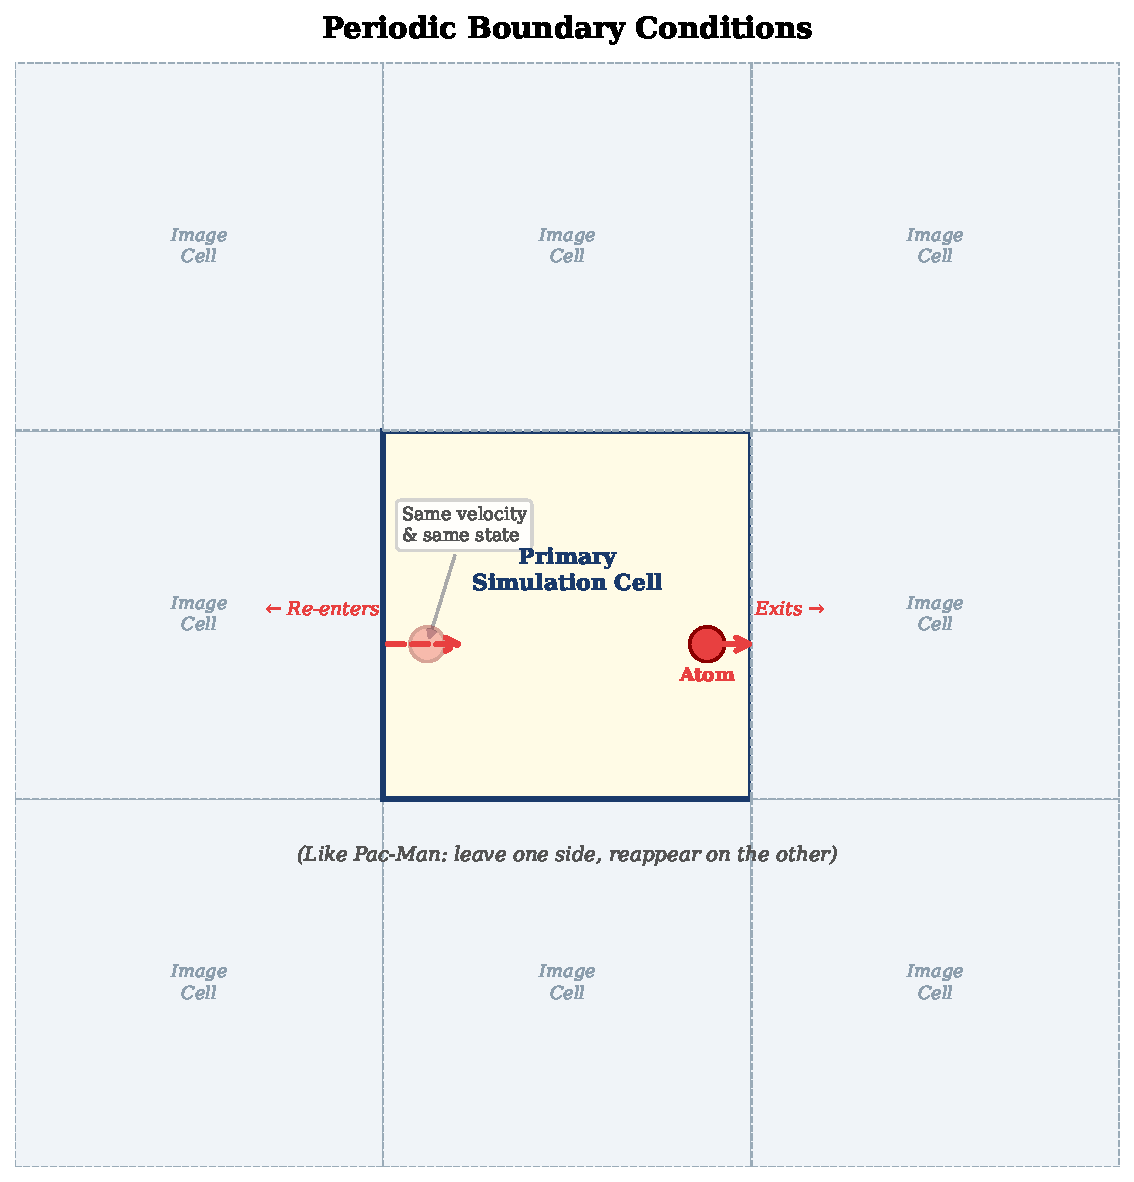
\includegraphics[width=0.72\linewidth]{figures/pbc_schematic.pdf}
    \caption{Periodic Boundary Conditions illustrated in 2D. The central yellow cell is the primary simulation cell; dashed cells are identical image replicas tiling all space. When the red atom exits the right boundary, it immediately re-enters from the left with the same velocity, keeping the total particle count constant. (credit to Claude for the image)}
    \label{fig:pbc}
\end{figure}

\subsubsection{What Is the Minimum Image Convention and Why Do We Apply It?}

Periodic Boundary Conditions solve the surface effect problem, but they introduce a new computational challenge: by definition, PBC creates an infinite array of replica cells extending throughout all of space. Naively, this means every atom in the primary cell must interact with infinitely many copies of every other atom in the universe. Without a system to limit these interactions, the simulation becomes mathematically impossible.

The Minimum Image Convention (MIC) is the \emph{filter} that makes PBC computationally feasible and physically correct. The MIC states a simple rule: when calculating the interaction between any two atoms, use only the \emph{nearest periodic image} of each pair. In practice, this means:

\begin{enumerate}
    \item Calculate the distance vector between atoms $i$ and $j$ in the primary cell.
    \item Apply periodic wrapping: if the distance component along any axis exceeds $L/2$, fold it back across the boundary to find the shortest path through the periodic lattice.
    \item Use this shortest distance to compute the potential energy and forces.
\end{enumerate}

\begin{figure}[H]
    \centering
    \begin{tikzpicture}[scale=1.2]
        % Draw adjacent image cells (dashed)
        \draw[gray!50, dashed] (-6,-2) rectangle (-2,2);
        \draw[gray!50, dashed] (2,-2) rectangle (6,2);
        \node[gray, font=\scriptsize] at (4, -1.7) {Image Cell};
        \node[gray, font=\scriptsize] at (-4, -1.7) {Image Cell};

        % Draw primary central cell (solid)
        \draw[thick, blue!80!black] (-2,-2) rectangle (2,2);
        \node[blue!80!black, font=\scriptsize] at (0, -1.7) {Primary Cell};

        % Box dimension L
        \draw[<->, thick] (-2, -2.3) -- (2, -2.3) node[midway, below] {$L$};

        % Atoms
        \filldraw[blue] (1.2, 0.4) circle (0.1) node[above right] {$i$};
        \filldraw[red] (-1.4, -0.3) circle (0.1) node[above left] {$j$};

        % Image atom
        \filldraw[red!40] (2.6, -0.3) circle (0.1) node[right, font=\small] {image $j'$};

        % Vectors
        \draw[->, red, thick, dashed] (1.2, 0.4) -- (-1.4, -0.3) node[midway, above, sloped, font=\scriptsize] {naive distance};
        \draw[->, green!60!black, thick] (1.2, 0.4) -- (2.6, -0.3) node[midway, below, sloped, font=\scriptsize] {MIC distance};
    \end{tikzpicture}
    \caption{Visualising the Minimum Image Convention (MIC). Atom $i$ interacts with the nearest periodic image $j'$, taking the shortest path across the boundary rather than the longer naive distance to the primary atom $j$.}
    \label{fig:mic_visual}
\end{figure}

A key subtlety: PBC and MIC work together correctly only if the simulation cell is large enough that the periodic images do not interfere with each other. This requires the interaction cutoff $r_c$ to satisfy $r_c \leq L/2$. This is discussed in detain in section \ref{sec:mic_constraint}.

\subsection{How Is It Implemented?}

\subsubsection{Periodic Boundary Wrapping}

After each integration step, any atom whose coordinate has drifted outside $[0, L)$ is wrapped back using the modulo operation:
\begin{equation}
    \mathbf{r}_i \leftarrow \mathbf{r}_i \bmod L
    \label{eq:pbc_wrap}
\end{equation}
This is equivalent to the conditional logic ($x > L \Rightarrow x - L$; $x < 0 \Rightarrow x + L$) but handles arbitrarily large displacements in a single line.

\subsubsection{Minimum Image Convention}
\label{sec:mic}

\begin{equation}
    dx_{ij} = x_i - x_j - L \cdot \mathrm{round}\!\left(\frac{x_i - x_j}{L}\right)
    \label{eq:mic}
\end{equation}
The rounding step identifies which periodic image of atom $j$ is closest to atom $i$ and shifts the distance accordingly. By construction, $dx_{ij} \in (-L/2,\, L/2]$, meaning the result is always the shortest path between the two atoms, whether that path goes through a wall or not.

\subsubsection{Cutoff Constraint}
\label{sec:mic_constraint}

The Minimum Image Convention (MIC) operates on a fundamental assumption: a particle interacts with only the single closest periodic image of any other particle. For this assumption to remain physically valid, the interaction cutoff radius must satisfy:
\begin{equation}
    r_c \leq \frac{L}{2}
    \label{eq:cutoff_constraint}
\end{equation}

If $r_c > L/2$, the physical "sphere of influence" around a particle becomes large enough to span across the periodic boundaries. As illustrated in Figure~\ref{fig:cutoff_constraint}, this causes the cutoff sphere to encompass multiple images of the exact same neighbour. Because the MIC algorithm mathematically truncates the distance to only the single nearest image, any secondary images falling within the $r_c$ range are artificially ignored. This creates a severe physical inconsistency where valid forces are discarded, leading to incorrect dynamics. 

In our simulation, $r_c^* = 2.5$ and the box length is $L^* \approx 6.71$ (for $n_\text{cells} = 4$, $\rho^* = 0.8442$). This yields $L/2 \approx 3.35$. Since $3.35 > 2.5$, the constraint is safely satisfied, ensuring no particle self-interacts or sees multiple images of its neighbours.

\begin{figure}[H]
    \centering
    \begin{tikzpicture}[scale=1.2]
        % Draw adjacent image cells (dashed)
        \draw[gray!50, dashed] (-6,-2) rectangle (-2,2);
        \draw[gray!50, dashed] (2,-2) rectangle (6,2);

        % Draw primary central cell (solid)
        \draw[thick, blue!80!black] (-2,-2) rectangle (2,2);
        \node[blue!80!black, font=\scriptsize] at (0, -1.7) {Primary Cell};

        % Center atom i
        \filldraw[blue] (0.6, 0) circle (0.1) node[above right] {$i$};

        % Atom j and its image
        \filldraw[red] (1.7, 0) circle (0.1) node[right] {$j$};
        \filldraw[red!40] (-2.3, 0) circle (0.1) node[left] {image $j'$};

        % L/2 boundaries
        \draw[<->, gray!80, thick] (-2, -2.3) -- (0, -2.3) node[midway, below, font=\scriptsize] {$L/2$};
        \draw[<->, gray!80, thick] (0, -2.3) -- (2, -2.3) node[midway, below, font=\scriptsize] {$L/2$};

        % Safe cutoff (Green)
        \draw[green!60!black, thick, dashed] (0.6, 0) circle (1.3);
        \draw[->, green!60!black] (0.6,0) -- (0.6, 1.3) node[midway, left, font=\scriptsize] {$r_c$};
        \node[green!60!black, font=\scriptsize, align=center] at (0.6, 1.6) {Safe: $r_c \leq L/2$ \\ (sees $j$ only)};

        % Unsafe cutoff (Red)
        \draw[red, thick, dashed] (0.6, 0) circle (3.1);
        \node[red, font=\scriptsize, align=center] at (0.6, 3.4) {Unsafe: $r_c > L/2$ \\ (sphere overlaps $j$ AND $j'$)};
    \end{tikzpicture}
    \caption{Visualizing the Cutoff Constraint. If the interaction cutoff $r_c$ exceeds $L/2$, the physical interaction sphere around atom $i$ encompasses both the primary atom $j$ and its periodic image $j'$. The MIC algorithm breaks down under these conditions, as it is designed to evaluate only a single unique pair interaction.}
    \label{fig:cutoff_constraint}
\end{figure}
\subsubsection{FCC Lattice Generation}

The simulation box length is determined from the target reduced number density:
\begin{equation}
    L = \left(\frac{N}{\rho^*}\right)^{1/3}, \quad N = 4\,n_\text{cells}^3
    \label{eq:box_length}
\end{equation}
A single FCC unit cell of side $a = L / n_\text{cells}$ contains four atoms at basis positions:
\begin{equation}
    \mathbf{b}_1 = (0,\,0,\,0),\quad
    \mathbf{b}_2 = \tfrac{a}{2}(1,\,1,\,0),\quad
    \mathbf{b}_3 = \tfrac{a}{2}(1,\,0,\,1),\quad
    \mathbf{b}_4 = \tfrac{a}{2}(0,\,1,\,1)
    \label{eq:fcc_basis}
\end{equation}
The full lattice is built by translating this unit cell to all $n_\text{cells}^3$ positions.

\newpage
\subsection{Test Results}

\subsubsection{FCC Lattice: Visualisation}

Figure~\ref{fig:fcc_lattice} shows the FCC lattice generated by \texttt{generate\_fcc\_lattice} with $n_\text{cells} = 3$ and $\rho^* = 4.0$ (a denser packing chosen for visual clarity). The resulting $N = 108$ atoms and box length $L = 3.0$ produce a clear FCC pattern. The characteristic feature of FCC (atoms at face centres offset by $a/2$ from corner atoms) is visible in the regular diagonal arrangements across each face of the cube.

\begin{figure}[H]
    \centering
    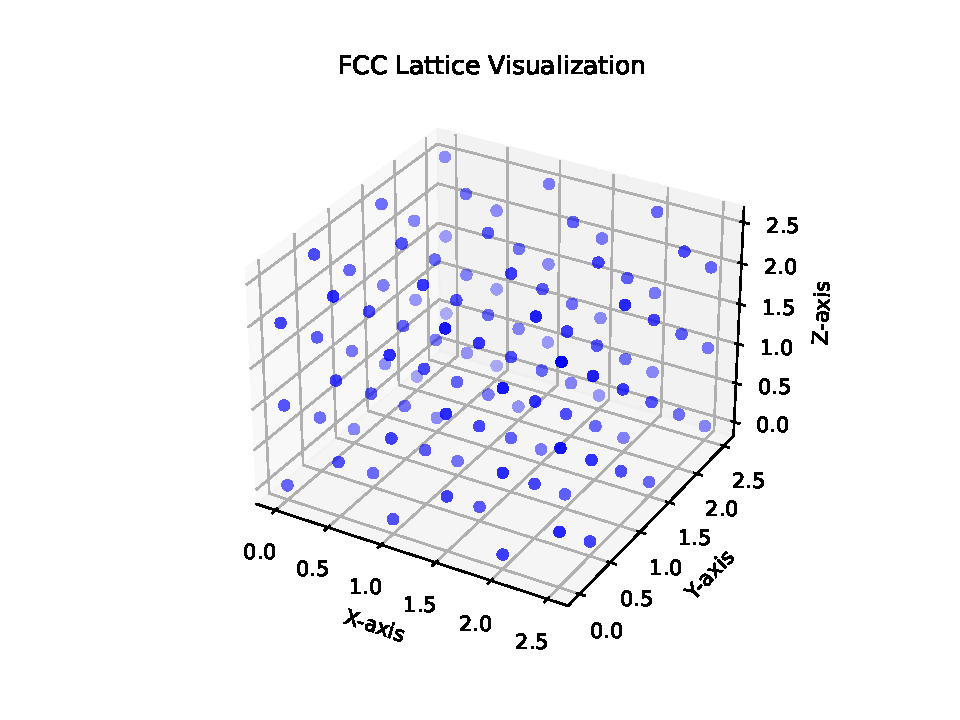
\includegraphics[width=0.62\linewidth]{figures/fcc_lattice.pdf}
    \caption{FCC lattice generated by \texttt{generate\_fcc\_lattice} with $n_\text{cells} = 3$, $\rho^* = 4.0$, giving $N = 108$ atoms in a box of $L = 3.0\,\sigma$. }
    \label{fig:fcc_lattice}
\end{figure}

To further verify the structural integrity of the generated geometry, orthogonal planar projections of the lattice onto the XY, YZ, and ZX planes are presented in Figure~\ref{fig:fcc_projections}. When an FCC structure is viewed precisely along any principal axis, the combination of corner and face-centred atoms aligns to form a regular 2D square grid with a spacing of exactly half the lattice constant ($a/2$). For our system with $L = 3.0$ and $n_\text{cells} = 3$, the lattice constant is $a = 1.0$. The projections correctly demonstrate atoms appearing at precise $0.5$ intervals along all axes, confirming the accurate spatial distribution and periodic boundaries of the setup.

\begin{figure}[H]
    \centering
    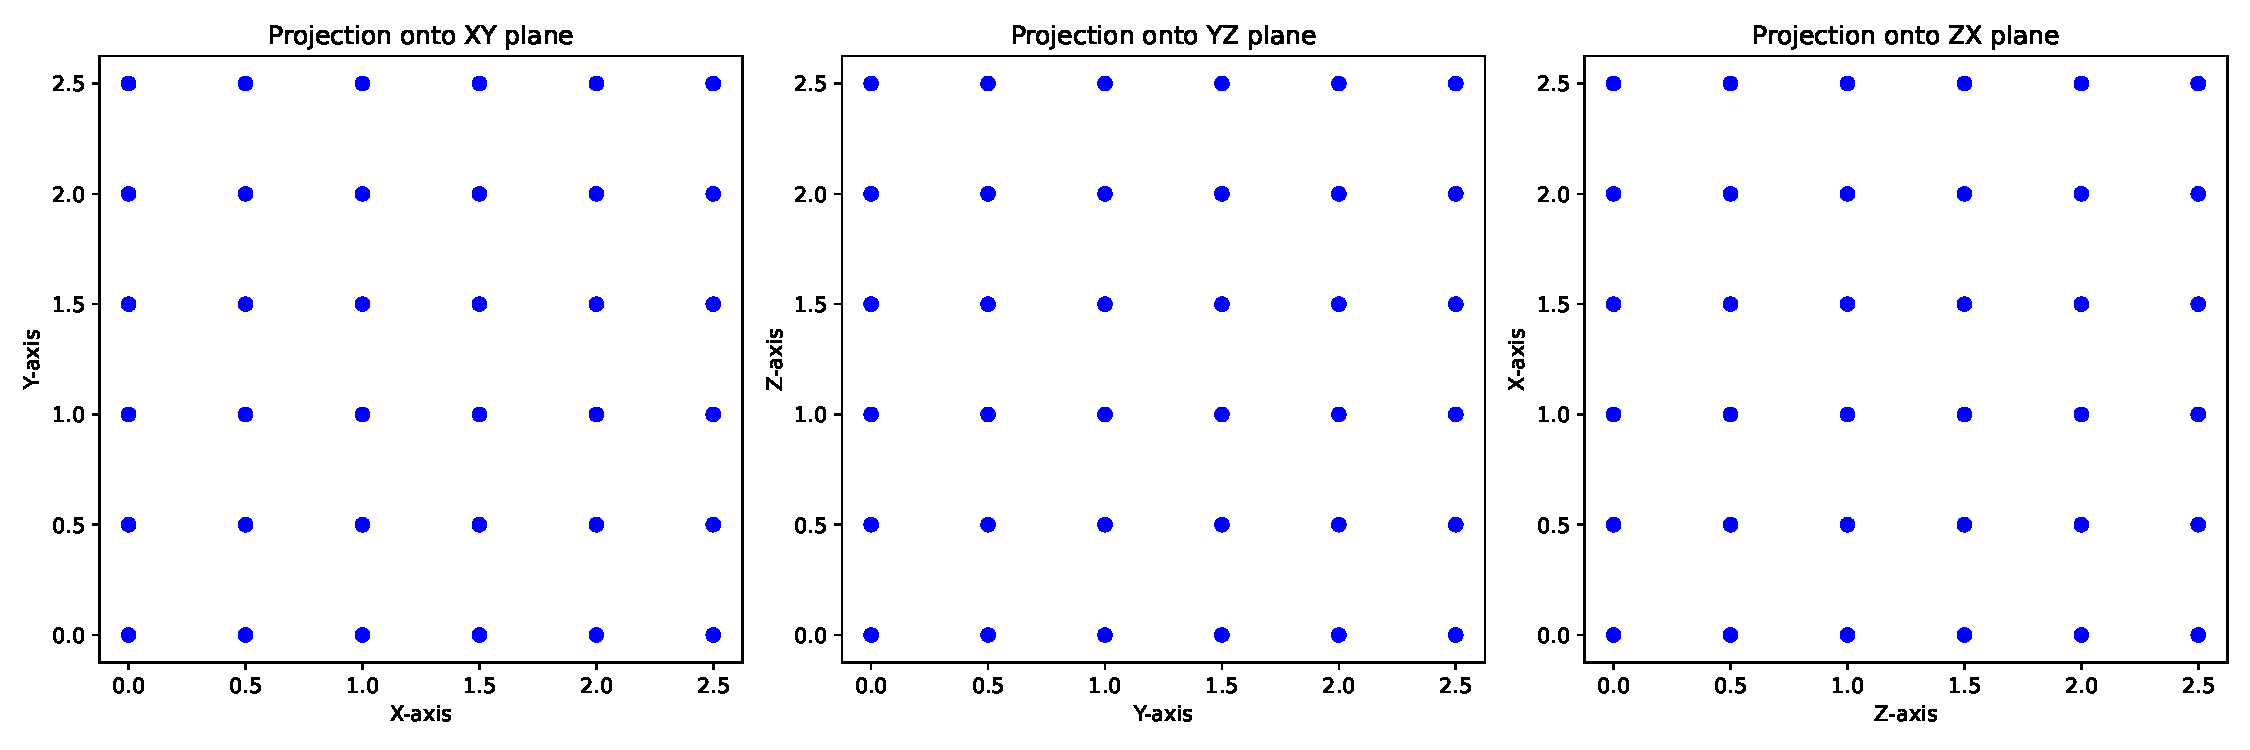
\includegraphics[width=\linewidth]{figures/fcc_lattice_2d_projection.pdf}
    \caption{Orthogonal projections of the simulated FCC lattice onto the XY, YZ, and ZX planes. The uniform grid with spacing $0.5\,\sigma$ confirms the correct structural implementation and the characteristic $a/2$ atomic offsets of the face-centred cubic geometry.}
    \label{fig:fcc_projections}
\end{figure}


\subsubsection{Minimum Image Convention: Visualisation and Test}
\label{sec:mic_test}

Figure~\ref{fig:mic} illustrates the application of the \texttt{apply\_minimum\_image} algorithm in a 2D system, verifying its ability to correctly fold coordinates across periodic boundaries.

In this test case, the simulation box has a length of $L = 10$, spanning from $0$ to $10$ along both axes. Atom 1 (the reference atom, shown in blue) is located at the center $\mathbf{r}_1 = (5, 5)$. Atom 2 (shown in red) has a raw coordinate of $\mathbf{r}_2 = (11, 4)$, placing it completely outside the primary simulation box.

The naive, direct displacement vector from Atom 1 to Atom 2 is:
\begin{equation*}
    \Delta\mathbf{r}_{\text{raw}} = \mathbf{r}_2 - \mathbf{r}_1 = (11 - 5, 4 - 5) = (6, -1)
\end{equation*}

Because the magnitude of the $x$-displacement ($\Delta x = 6$) is strictly greater than $L/2 = 5$, it violates the minimum image criteria. The MIC algorithm corrects this by applying the rounding formula to find the shortest path across the periodic boundary:
\begin{equation*}
    dx_{\text{MIC}} = 6 - 10 \cdot \mathrm{round}\left(\frac{6}{10}\right) = 6 - 10 \times 1 = -4
\end{equation*}
The $y$-displacement ($\Delta y = -1$) is already within the $[-5, 5]$ bounds, so it remains unchanged ($dy_{\text{MIC}} = -1 - 10 \times 0 = -1$). The resulting MIC displacement vector is $\Delta\mathbf{r}_{\text{MIC}} = (-4, -1)$.

As shown in Figure~\ref{fig:mic}, adding this corrected displacement vector to Atom 1 yields the effective position of Atom 2's closest periodic image: $(5, 5) + (-4, -1) = (1, 4)$. The solid green line accurately represents this minimum image distance, confirming that the code successfully maps the atom to its correct periodic representation (the green dot) within the primary interaction neighbourhood.

\begin{figure}[H]
    \centering
    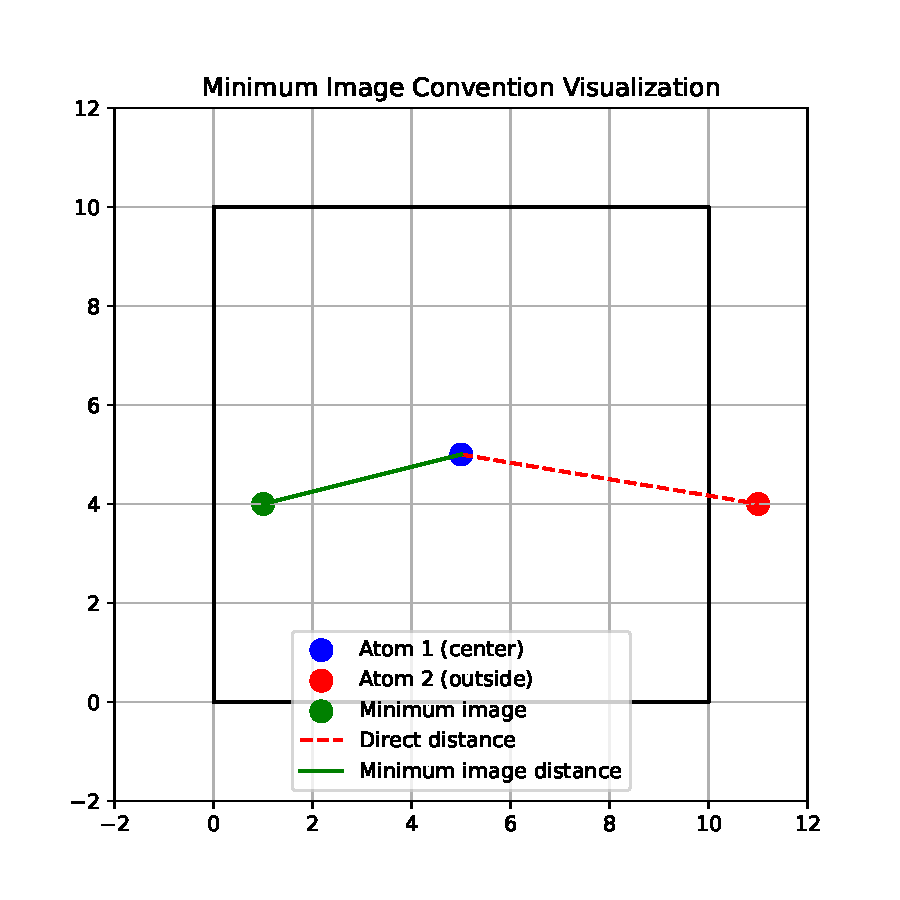
\includegraphics[width=0.8\linewidth]{figures/minimum_image_convention.pdf}
    \caption{Minimum Image Convention (MIC) visualization in a 2D box of $L = 10$. Atom 1 is located at $(5,5)$ and Atom 2 is outside the box at $(11,4)$. The direct distance (dashed red line) yields an $x$-displacement of $6$, exceeding $L/2$. The MIC algorithm folds the calculation across the periodic boundary, correctly identifying the minimum image of Atom 2 at $(1,4)$ (green dot). The solid green line represents the true shortest interaction vector $\Delta\mathbf{r}_{\text{MIC}} = (-4, -1)$ computed by the algorithm.}
    \label{fig:mic}
\end{figure}